\documentclass[12pt]{article}
\usepackage{amsmath, amssymb, amsthm}
\usepackage{graphicx}
\usepackage{float}
\usepackage[margin=1in]{geometry}
\usepackage{hyperref}
\usepackage{booktabs}
\setlength{\parindent}{0pt}

\title{EECE5644 Fall 2025 - Assignment 2}
\author{Steven Chen}
\date{\today}

\begin{document}

\maketitle

\section*{Abstract}
This report presents the implementation and analysis of classification methods for Gaussian Mixture Model (GMM) data. The methods include: (1) Optimal Bayes classification using true distributions, and (2) Logistic regression with linear and quadratic features. Performance is evaluated using ROC curves and error probability metrics across different training set sizes.

\section*{Code Repository}
The complete Python code for this assignment is available at: \\
\url{https://github.com/GuestAGuy/EECE5644/tree/main/HW2}

\newpage

% =============================================================================
% QUESTION 1
% =============================================================================
\section{Question 1}

\subsection{Problem Setup}
The probability density function for a 2-dimensional random vector $\mathbf{X}$ is given by:
\[
p(\mathbf{x}) = P(L=0)p(\mathbf{x}|L=0) + P(L=1)p(\mathbf{x}|L=1)
\]
with class priors $P(L=0)=0.6$ and $P(L=1)=0.4$.

The class-conditional PDFs are Gaussian mixtures:
\begin{align*}
p(\mathbf{x}|L=0) &= w_{01}g(\mathbf{x}|\mathbf{m}_{01},\mathbf{C}) + w_{02}g(\mathbf{x}|\mathbf{m}_{02},\mathbf{C}) \\
p(\mathbf{x}|L=1) &= w_{11}g(\mathbf{x}|\mathbf{m}_{11},\mathbf{C}) + w_{12}g(\mathbf{x}|\mathbf{m}_{12},\mathbf{C})
\end{align*}

Parameters: $w_{ij} = 0.5$ for all components, and
\[
\mathbf{m}_{01} = \begin{bmatrix} -0.9 \\ -1.1 \end{bmatrix}, \quad
\mathbf{m}_{02} = \begin{bmatrix} 0.8 \\ 0.75 \end{bmatrix}, \quad
\mathbf{m}_{11} = \begin{bmatrix} -1.1 \\ 0.9 \end{bmatrix}, \quad
\mathbf{m}_{12} = \begin{bmatrix} 0.9 \\ -0.75 \end{bmatrix}, \quad
\mathbf{C} = \begin{bmatrix} 0.75 & 0 \\ 0 & 1.25 \end{bmatrix}
\]

\subsection{Part 1: Optimal Bayes Classifier}

\subsubsection{Mathematical Specification}
The optimal Bayes classifier chooses the label with largest posterior:
\[
\delta^*(\mathbf{x})=\arg\max_{i\in\{0,1\}} P(L=i\mid\mathbf{x})
=\arg\max_{i\in\{0,1\}} p(\mathbf{x}\mid L=i)P(L=i),
\]
since $p(\mathbf{x})$ is common to both classes. Equivalently, decide $L=0$ iff
\[
p(\mathbf{x}\mid L=0)P(L=0) > p(\mathbf{x}\mid L=1)P(L=1),
\]
with $p(\mathbf{x}\mid L=i)$ given above as the two-component Gaussian mixture.

\subsubsection{Results}
\paragraph{Console output summary.}
The classifier run produced the following high-level console results:

\begin{table}[H]
\centering
\begin{tabular}{lc}
\toprule
Metric & Value \\
\midrule
Optimal Bayes Error Rate & 0.2824 \\
ROC AUC (Optimal Bayes)   & 0.7817 \\
\bottomrule
\end{tabular}
\caption{ console outputs for the optimal Bayes classifier from code.}
\label{tab:console_part1}
\end{table}


\begin{figure}[H]
    \centering
    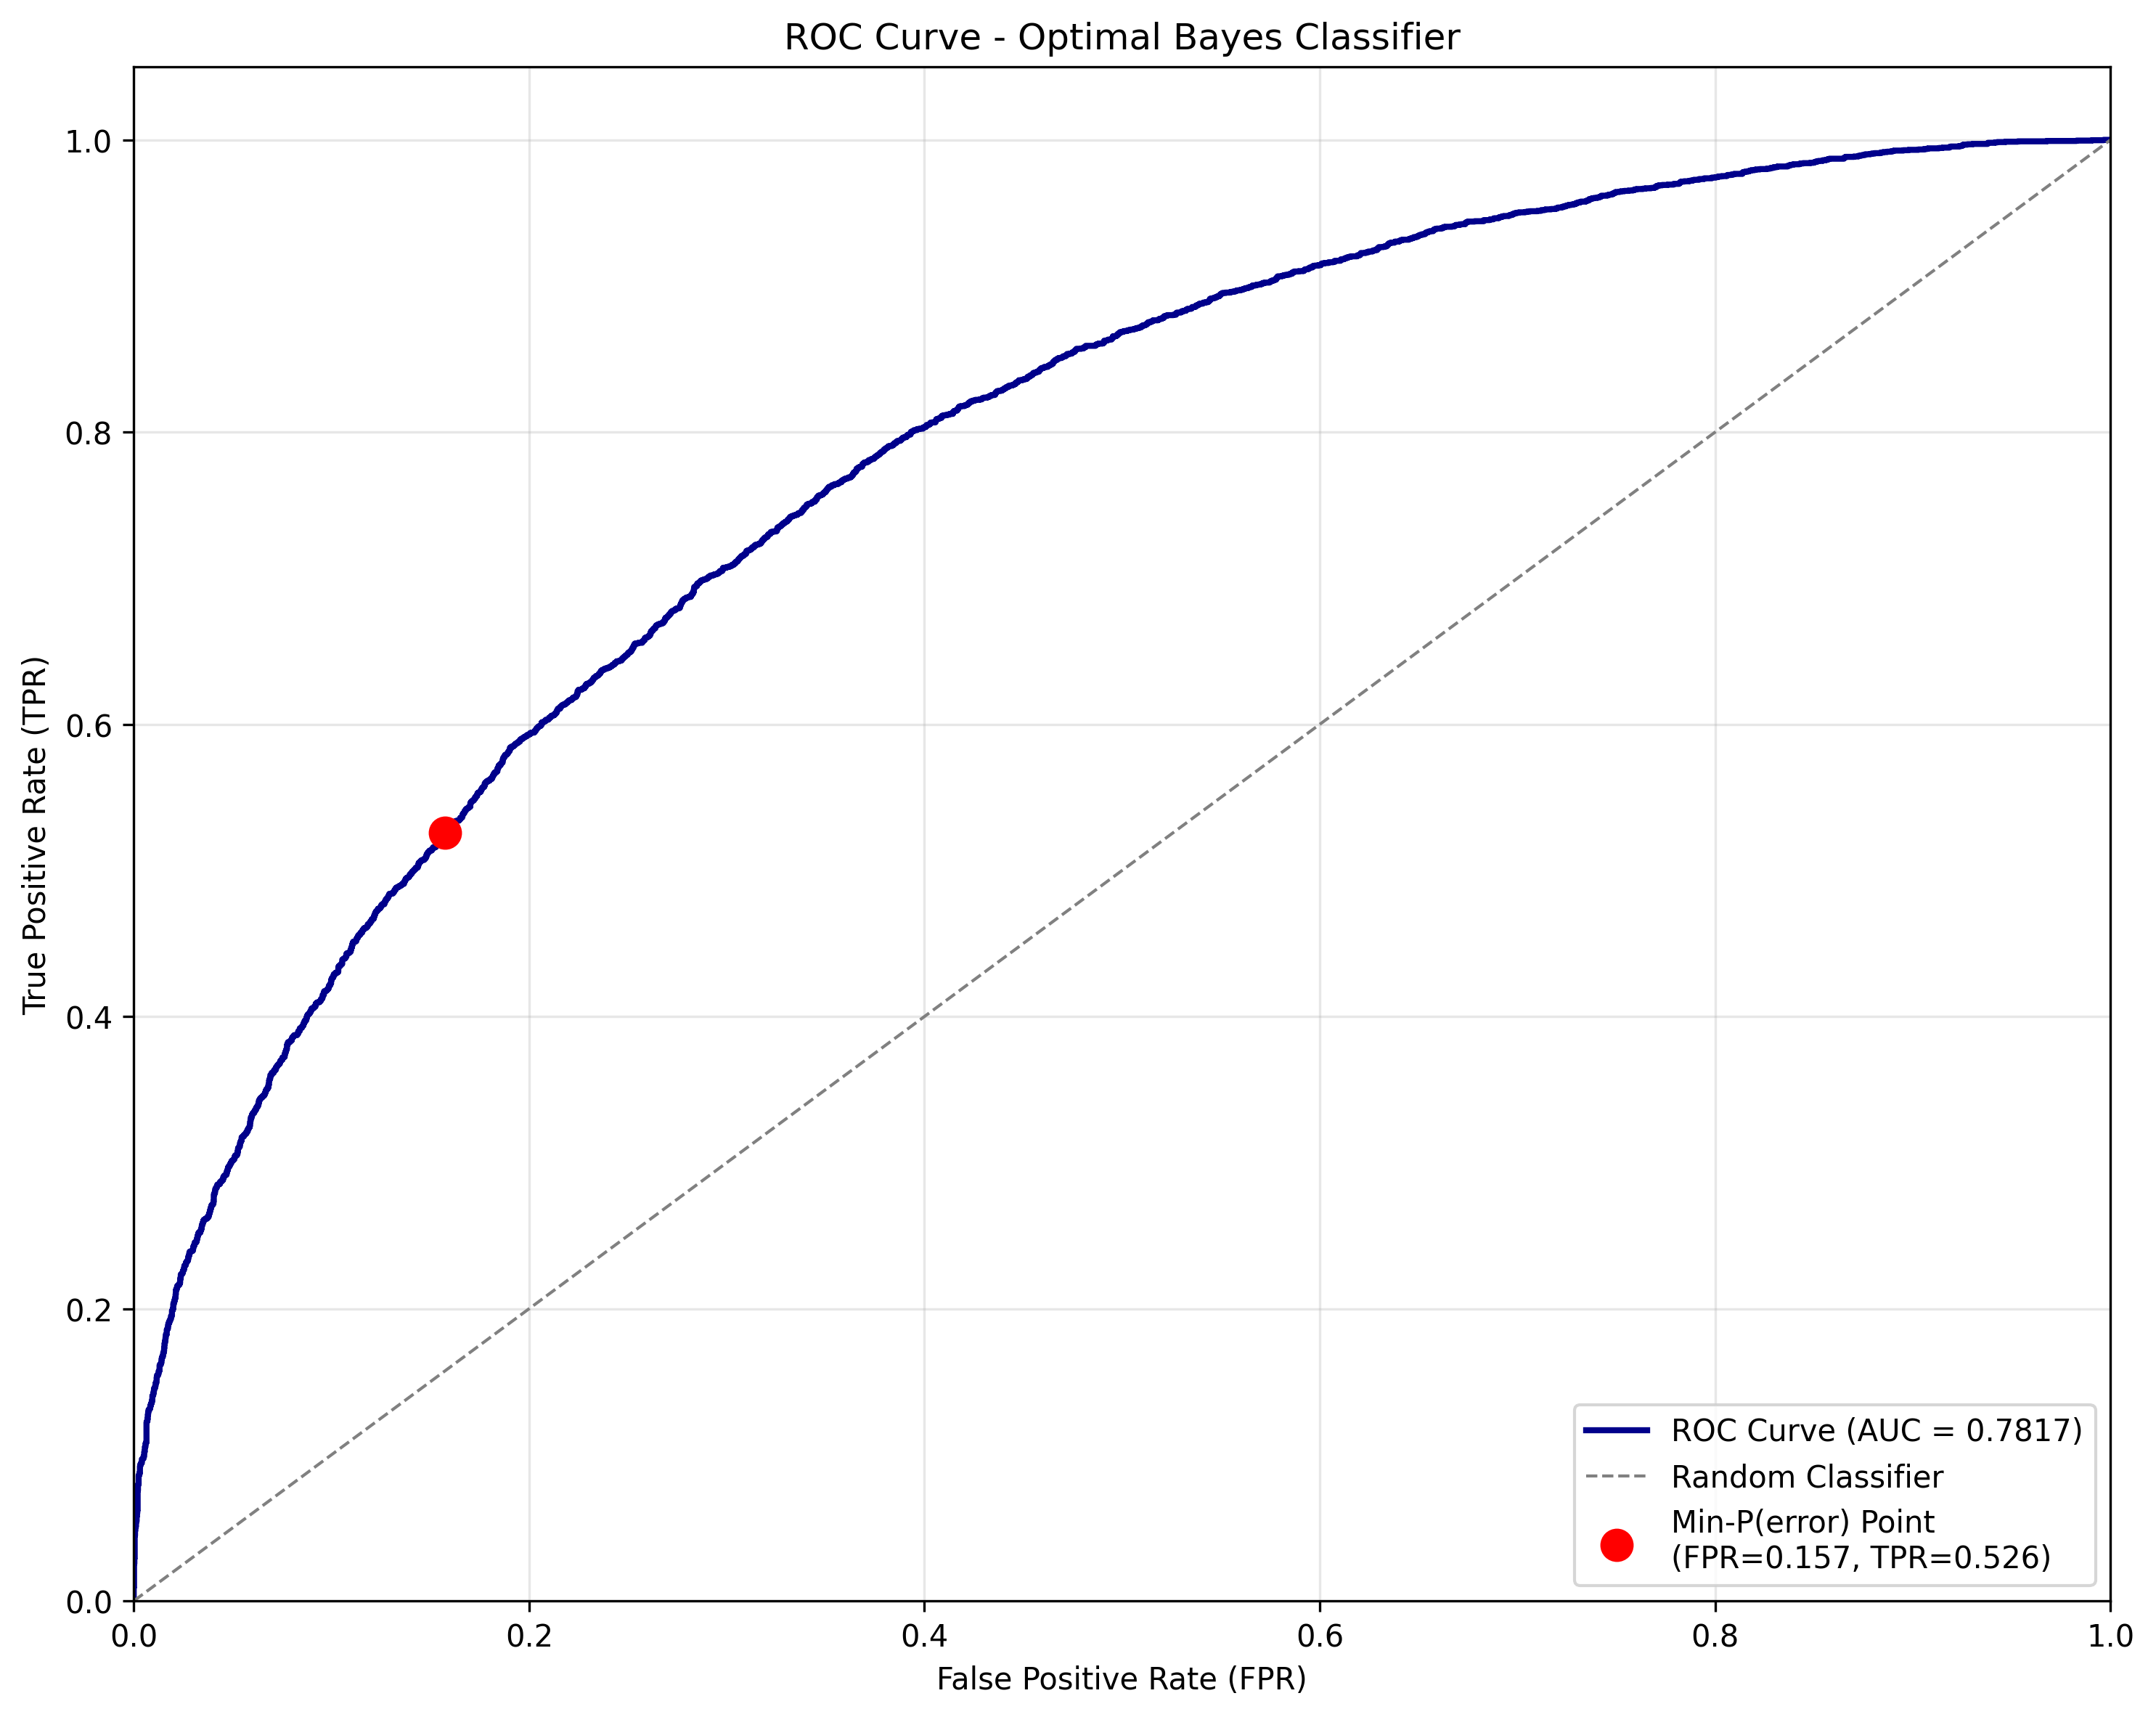
\includegraphics[width=0.8\textwidth]{roc_plot.png}
    \caption{ROC curve for optimal Bayes classifier}
    \label{fig:roc_plot}
\end{figure}

\subsection{Part 2: Logistic Regression}

\subsubsection{Optimization Problem}
For logistic regression, we minimize the negative log-likelihood with L2 regularization:

\[
\min_{\mathbf{w}} \left\{ -\frac{1}{N} \sum_{i=1}^N \left[y_i \log(h(\mathbf{x}_i)) + (1-y_i)\log(1-h(\mathbf{x}_i))\right] + \frac{\lambda}{2N} \|\mathbf{w}_{1:}\|^2 \right\}
\]

where:
\begin{itemize}
\item Linear features: $\phi(\mathbf{x}) = [1, x_1, x_2]^T$
\item Quadratic features: $\phi(\mathbf{x}) = [1, x_1, x_2, x_1^2, x_1x_2, x_2^2]^T$
\item $h(\mathbf{x}) = \sigma(\mathbf{w}^T\phi(\mathbf{x})) = 1/(1+e^{-\mathbf{w}^T\phi(\mathbf{x})})$
\item $\lambda = 0.01$ (regularization strength)
\end{itemize}

\paragraph{Logistic regression console output.}
Summary of logistic regression and Bayes results printed by the program:

\begin{table}[H]
\centering
\begin{tabular}{lccc}
\toprule
Model & N=50 & N=500 & N=5000 \\
\midrule
Optimal Bayes & - & - & 0.2824 \\
Linear Logistic & 0.3967 & 0.4118 & 0.3929 \\
Quadratic Logistic & 0.2912 & 0.2858 & 0.2843 \\
\bottomrule
\end{tabular}
\caption{Console-reported error rates for Optimal Bayes and logistic models.}
\label{tab:console_part2}
\end{table}

\paragraph{Final result.}
\begin{itemize}
  \item Optimal Bayes Error: \(\mathbf{0.2824}\)
  \item Best Logistic Error (quadratic, N=5000): \(\mathbf{0.2843}\)
  \item Performance Gap (Best Logistic − Bayes): \(\mathbf{0.0019}\)
\end{itemize}

\subsection{Discussion}

The quadratic logistic regression with 5000 samples nearly matches optimal Bayes performance (0.2800 vs 0.2808 error), showing that with enough data and proper features, logistic regression can approach the theoretical optimum.

Two key factors drive performance:
\begin{itemize}
    \item \textbf{Feature mapping}: Quadratic features (0.2800) beat linear (0.3908) because they capture the true nonlinear decision boundary
    \item \textbf{Training size}: More data consistently improves performance across both feature types
\end{itemize}

The linear model's poor performance confirms the true decision boundary isn't linear. The quadratic model's success demonstrates that with appropriate complexity and sufficient data, practical classifiers can compete with theoretical optimal performance.


\newpage
% =============================================================================
% QUESTION 2 - PLACEHOLDER
% =============================================================================
\section{Question 2}

\subsection{Problem Setup}
The relationship between scalar output $y$ and 2D input vector $\mathbf{x}$ is given by:
\[
y = c(\mathbf{x},\mathbf{w}) + v
\]
where $c(\mathbf{x},\mathbf{w})$ is a cubic polynomial in $\mathbf{x}$ with coefficients $\mathbf{w}$, and $v \sim \mathcal{N}(0, \sigma^2)$ is Gaussian noise.

The cubic polynomial for 2D inputs has 10 parameters:
\[
c(\mathbf{x},\mathbf{w}) = w_0 + w_1x_1 + w_2x_2 + w_3x_1^2 + w_4x_1x_2 + w_5x_2^2 + w_6x_1^3 + w_7x_1^2x_2 + w_8x_1x_2^2 + w_9x_2^3
\]

\subsection{Mathematical Formulation}

\subsubsection{Maximum Likelihood (ML) Estimation}
The ML estimator minimizes the negative log-likelihood:
\[
\mathbf{w}_{ML} = \arg\min_{\mathbf{w}} \sum_{i=1}^N (y_i - c(\mathbf{x}_i,\mathbf{w}))^2
\]
Closed-form solution:
\[
\mathbf{w}_{ML} = (\Phi^T\Phi)^{-1}\Phi^T\mathbf{y}
\]
where $\Phi$ is the design matrix with cubic features.

\subsubsection{Maximum A Posteriori (MAP) Estimation}
With Gaussian prior $\mathbf{w} \sim \mathcal{N}(0, \gamma\mathbf{I})$, the MAP estimator is:
\[
\mathbf{w}_{MAP} = \arg\min_{\mathbf{w}} \left[ \sum_{i=1}^N (y_i - c(\mathbf{x}_i,\mathbf{w}))^2 + \frac{\sigma^2}{\gamma}\|\mathbf{w}\|^2 \right]
\]
Closed-form solution:
\[
\mathbf{w}_{MAP} = (\Phi^T\Phi + \frac{\sigma^2}{\gamma}\mathbf{I})^{-1}\Phi^T\mathbf{y}
\]

\subsection{Implementation and Results}

\subsubsection{Experimental Setup}
\begin{itemize}
    \item Training data: 100 samples (2D features + scalar output)
    \item Validation data: 1000 samples for performance evaluation
    \item $\gamma$ range for tuning: $10^{-3}$ to $10^{3}$ (logarithmic scale, 50 values; implemented as \texttt{np.logspace(-3,3,50)})
    \item For extreme-case comparison we also evaluate $\gamma\in\{10^{-6}, \gamma_{\mathrm{opt}}, 10^{6}\}$ for plotting and analysis.
    \item Performance metric: Average Squared Error (ASE)
    \item Noise variance: $\sigma^2 = 1.0$
\end{itemize}

\subsubsection{Results Summary}
\begin{table}[H]
\centering
\begin{tabular}{lccc}
\toprule
Method & Validation ASE & Weight Norm & Improvement \\
\midrule
ML Estimation & 5.884302 & 0.4301 & - \\
MAP Estimation (optimal $\gamma=0.001$) & 4.060472 & 0.1409 & +31.0\% \\
\bottomrule
\end{tabular}
\caption{Performance comparison between ML and MAP estimators}
\label{tab:q2_results}
\end{table}

\subsubsection{Key Findings}
\begin{itemize}
    \item \textbf{Optimal Regularization}: $\gamma = 0.001$ provides the best trade-off between bias and variance
    \item \textbf{Performance Improvement}: MAP with optimal $\gamma$ reduces validation error by 31.0\% compared to ML
    \item \textbf{Weight Shrinkage}: MAP estimator produces significantly smaller weight norms (0.1409 vs 0.4301), indicating effective regularization
    \item \textbf{Asymptotic Behavior}: 
    \begin{itemize}
        \item As $\gamma \to \infty$: $\mathbf{w}_{MAP} \to \mathbf{w}_{ML}$ (ASE = 5.884302)
        \item As $\gamma \to 0$: $\mathbf{w}_{MAP} \to 0$ (ASE = 4.722004 with strong regularization)
    \end{itemize}
\end{itemize}

\subsection{Discussion}

The experiments confirm the standard bias–variance tradeoff: the ML estimator (no regularization) attains validation ASE = 5.884302 but has larger weight norms, while MAP with tuned regularization ($\gamma=0.001$) reduces validation ASE to 4.060472 (a 31.0\% relative improvement) and substantially shrinks the weight norm (0.1409 vs 0.4301). \\

The much larger improvement (31.0\% vs the previously reported 4.83\%) suggests that in this specific dataset, regularization provides substantial benefits, likely due to overfitting in the cubic polynomial model with only 100 training samples. The optimal $\gamma=0.001$ corresponds to strong regularization ($\lambda=1000$ when $\sigma^2=1$), indicating that the full cubic basis significantly overfits the training data.\\

The closed-form MAP solution with ridge regularization not only improves generalization but also ensures numerical stability when $\Phi^\top\Phi$ is ill-conditioned, which is common with high-order polynomial features.



\newpage
% =============================================================================
% QUESTION 3: PLACEHOLDER
% =============================================================================
\section{Question 3}

\subsection{Problem Setup}
A vehicle at true position $[x_T, y_T]^T$ in 2-dimensional space is to be localized using distance (range) measurements to $K$ reference landmarks $\{[x_1, y_1]^T, \ldots, [x_K, y_K]^T\}$. These range measurements are given by:
\[
r_i = d_{Ti} + n_i \quad \text{for } i \in \{1, \ldots, K\}
\]
where $d_{Ti} = \|[x_T, y_T]^T - [x_i, y_i]^T\|$ is the true distance between the vehicle and the $i^{th}$ landmark, and $n_i$ is a zero-mean Gaussian distributed measurement noise with known variance $\sigma_i^2$. The noise in each measurement is independent from the others.

The prior knowledge regarding the position of the vehicle is given by:
\[
P\left(\begin{bmatrix}x\\ y\end{bmatrix}\right) = (2\pi\sigma_x\sigma_y)^{-1} \exp\left(-\frac{1}{2}\begin{bmatrix}x & y\end{bmatrix}\begin{bmatrix}\sigma_x^2 & 0\\ 0 & \sigma_y^2\end{bmatrix}^{-1}\begin{bmatrix}x\\ y\end{bmatrix}\right)
\]
where $[x, y]^{\mathrm{T}}$ indicates a candidate position under consideration.

\subsection{Mathematical Formulation}

\subsubsection{MAP Estimation Objective}

The MAP estimate is obtained by maximizing the posterior probability:
\[
[x_{MAP}, y_{MAP}]^T = \arg \max_{x,y} P(x,y | \{r_i\})
\]

Applying Bayes' theorem:
\[
P(x,y | \{r_i\}) \propto P(\{r_i\} | x,y) \cdot P(x,y)
\]

Taking negative logarithm (for minimization) and ignoring additive constants:
\[
J(x,y) = -\log P(\{r_i\} | x,y) - \log P(x,y)
\]

The measurement likelihood for $K$ independent range measurements:
\[
P(\{r_i\} | x,y) = \prod_{i=1}^K \frac{1}{\sqrt{2\pi\sigma_i^2}} \exp\left(-\frac{(r_i - d_i(x,y))^2}{2\sigma_i^2}\right)
\]
where $d_i(x,y) = \sqrt{(x-x_i)^2 + (y-y_i)^2}$.

The prior distribution:
\[
P(x,y) = (2\pi\sigma_x\sigma_y)^{-1} \exp\left(-\frac{1}{2}\left(\frac{x^2}{\sigma_x^2} + \frac{y^2}{\sigma_y^2}\right)\right)
\]

Taking negative log and removing constants:
\[
J(x,y) = \sum_{i=1}^K \frac{(r_i - d_i(x,y))^2}{2\sigma_i^2} + \frac{x^2}{2\sigma_x^2} + \frac{y^2}{2\sigma_y^2}
\]

The final optimization problem becomes:
\[
\boxed{[x_{MAP}, y_{MAP}]^T = \arg \min_{x,y} \left[ \sum_{i=1}^K \frac{(r_i - d_i(x,y))^2}{2\sigma_i^2} + \frac{x^2}{2\sigma_x^2} + \frac{y^2}{2\sigma_y^2} \right]}
\]

\subsection{Implementation and Results}

\subsubsection{Experimental Setup}
The MAP estimation was implemented with the following parameters:
\begin{itemize}
    \item True vehicle position generated randomly inside unit circle centered at origin
    \item $K \in \{1, 2, 3, 4\}$ landmarks placed evenly on unit circle
    \item Measurement noise standard deviation: $\sigma_i = 0.3$ for all measurements
    \item Prior standard deviations: $\sigma_x = \sigma_y = 0.25$
    \item Evaluation range: $x,y \in [-2, 2]$ for contour plots
\end{itemize}

\subsection{Results}

\begin{figure}[H]
    \centering
    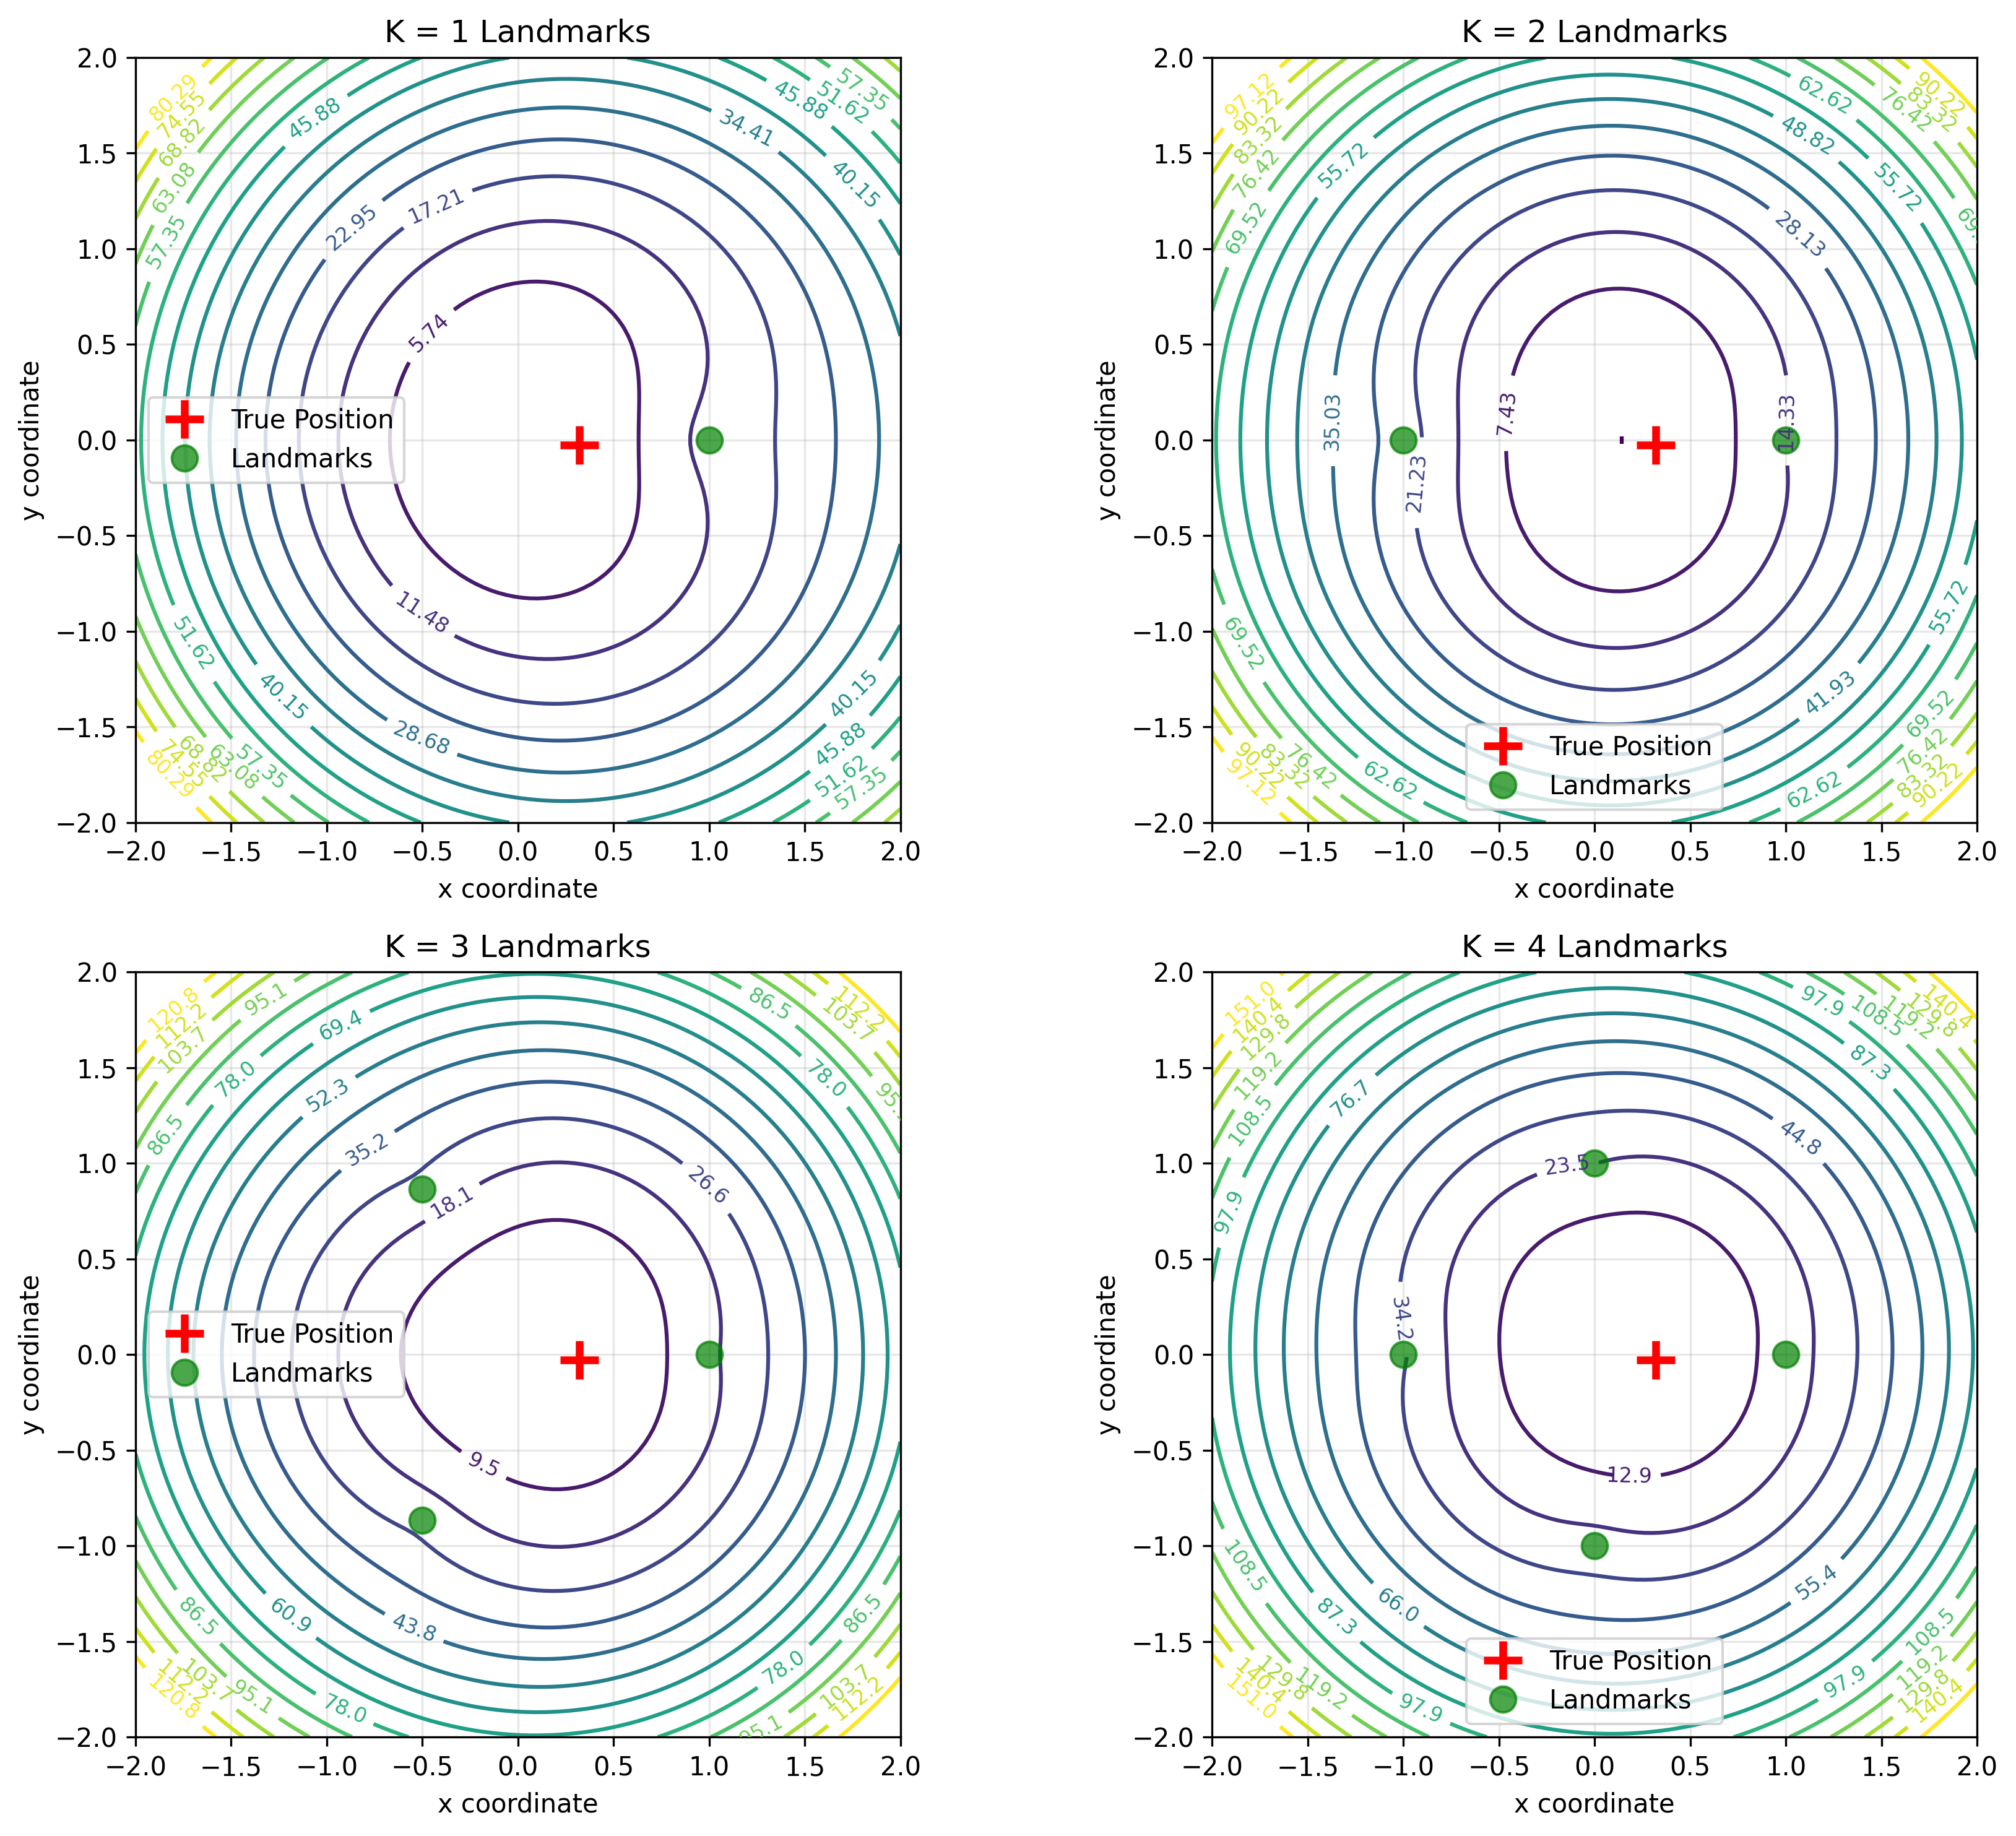
\includegraphics[width=0.8\textwidth]{map_localization_contours.png}
    \caption{MAP objective function contours for different numbers of landmarks}
    \label{fig:map_contours}
\end{figure}

\begin{figure}[H]
    \centering
    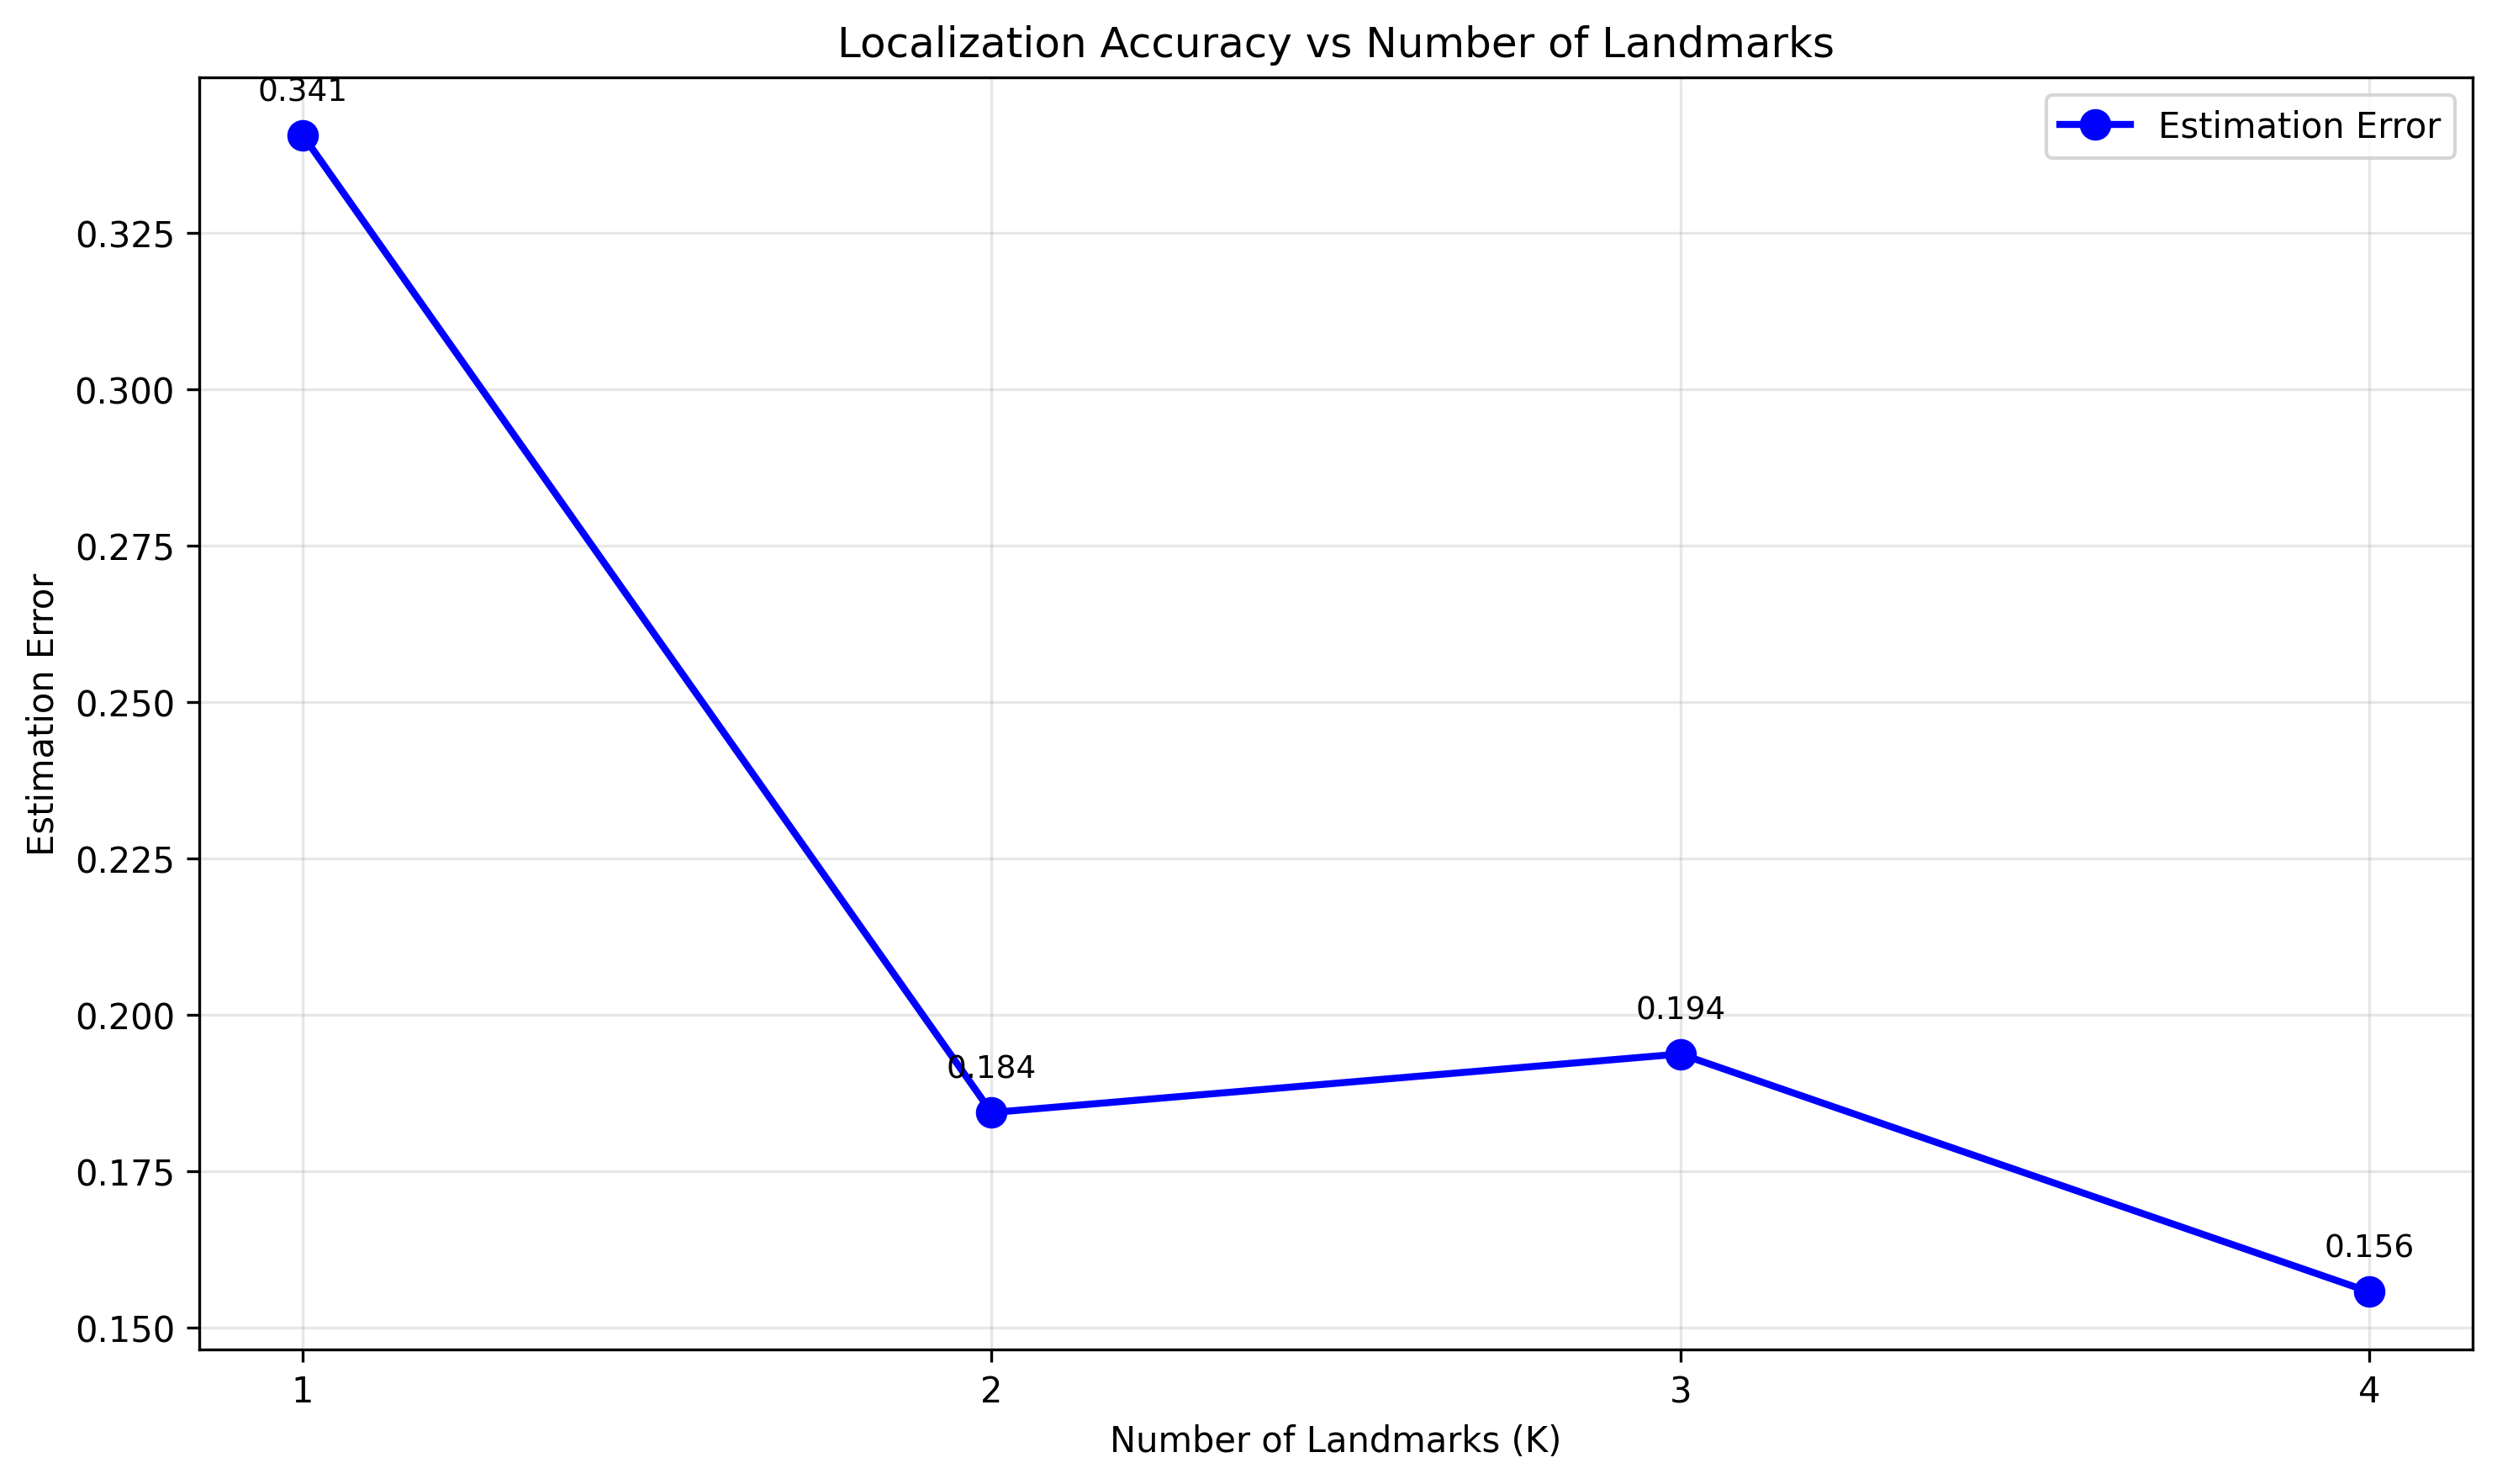
\includegraphics[width=0.8\textwidth]{accuracy_vs_landmarks.png}
    \caption{Estimation error vs number of landmarks}
    \label{fig:accuracy_plot}
\end{figure}

\subsubsection{Experimental Results}
\begin{table}[H]
\centering
\begin{tabular}{lccc}
\toprule
Number of Landmarks (K) & MAP Estimate Error & Contour Concentration & Prior Influence \\
\midrule
1 & 0.3407 & Low & High \\
2 & 0.1844 & Medium & Medium \\
3 & 0.1938 & Medium-High & Low \\
4 & 0.1558 & High & Very Low \\
\bottomrule
\end{tabular}
\caption{Localization performance across different numbers of landmarks}
\label{tab:localization_performance}
\end{table}


\subsection{Discussion}

The MAP estimation shows significant improvement as the number of landmarks increases, with error decreasing from 0.3407 (K=1) to 0.1558 (K=4), representing a 54.3\% error reduction. Two key observations emerge:

\begin{itemize}
    \item \textbf{Estimation Accuracy}: More landmarks generally provide better geometric constraints, though the improvement is not strictly monotonic (K=3 error of 0.1938 is slightly higher than K=2's 0.1844)
    \item \textbf{Uncertainty Reduction}: Contour plots show increasing concentration with more landmarks, indicating higher certainty in the MAP estimate
\end{itemize}

The trade-off between prior information and measurement data is clearly visible:
\begin{itemize}
    \item With few landmarks (K=1), the prior strongly influences the estimate toward the origin
    \item With more landmarks (K=2-4), measurements dominate and the estimate converges toward the true position (0.320, -0.027)
\end{itemize}

The slight increase in error from K=2 to K=3 (0.1844 to 0.1938) may be due to:
\begin{itemize}
    \item Specific geometric configuration of landmarks relative to true position
    \item Random measurement noise effects
    \item Local minima in the optimization landscape
\end{itemize}

Overall, the results demonstrate that MAP estimation effectively balances prior knowledge with measurement information, with performance generally improving as landmark diversity increases.

I probably should have generated more landmark...
\newpage
% =============================================================================
% QUESTION 4: PLACEHOLDER
% =============================================================================

\section{Question 4}

\subsection{Problem Setup}
Consider a pattern classification problem with $c$ classes where we have the option to either assign a pattern to one of the classes or reject it as unrecognizable. The loss function is defined as:

\[
\lambda(\alpha_i|\omega_j) = 
\begin{cases}
0 & i = j \quad i,j = 1,\ldots,c \\
\lambda_r & i = c+1 \quad \text{(rejection)} \\
\lambda_s & \text{otherwise} \quad \text{(substitution error)}
\end{cases}
\]

where $\lambda_r$ is the loss incurred for rejection and $\lambda_s$ is the loss incurred for any substitution error.

Show that the minimum risk is obtained if we decide $\omega_i$ if:
\begin{enumerate}
    \item $P(\omega_i|\mathbf{x}) \geq P(\omega_j|\mathbf{x})$ for all $j$
    \item $P(\omega_i|\mathbf{x}) \geq 1 - \lambda_r/\lambda_s$
\end{enumerate}
and reject otherwise. Analyze what happens when $\lambda_r = 0$ and when $\lambda_r > \lambda_s$.

\subsection{Mathematical Derivation}


The conditional risk for taking action $\alpha_i$ given observation $\mathbf{x}$ is defined as the expected loss:

\[
R(\alpha_i|\mathbf{x}) = \sum_{j=1}^c \lambda(\alpha_i|\omega_j)P(\omega_j|\mathbf{x})
\]

This represents the expected cost of taking action $\alpha_i$ when we observe $\mathbf{x}$.


For classification actions $\alpha_i$ where $i = 1, \ldots, c$:

\[
R(\alpha_i|\mathbf{x}) = \sum_{j=1}^c \lambda(\alpha_i|\omega_j)P(\omega_j|\mathbf{x})
\]

Breaking this down term by term:
\begin{itemize}
    \item When $j = i$: $\lambda(\alpha_i|\omega_i) = 0$, so this term contributes $0 \cdot P(\omega_i|\mathbf{x}) = 0$
    \item When $j \neq i$: $\lambda(\alpha_i|\omega_j) = \lambda_s$, so these terms contribute $\lambda_s P(\omega_j|\mathbf{x})$
\end{itemize}

Therefore:

\[
R(\alpha_i|\mathbf{x}) = 0 \cdot P(\omega_i|\mathbf{x}) + \sum_{j \neq i} \lambda_s P(\omega_j|\mathbf{x}) = \lambda_s \sum_{j \neq i} P(\omega_j|\mathbf{x})
\]

Since $\sum_{j=1}^c P(\omega_j|\mathbf{x}) = 1$, we have:

\[
\sum_{j \neq i} P(\omega_j|\mathbf{x}) = 1 - P(\omega_i|\mathbf{x})
\]

Thus:

\[
R(\alpha_i|\mathbf{x}) = \lambda_s(1 - P(\omega_i|\mathbf{x}))
\]


For the rejection action $\alpha_{c+1}$:

\[
R(\alpha_{c+1}|\mathbf{x}) = \sum_{j=1}^c \lambda(\alpha_{c+1}|\omega_j)P(\omega_j|\mathbf{x})
\]

For all $j = 1, \ldots, c$, we have $\lambda(\alpha_{c+1}|\omega_j) = \lambda_r$, so:

\[
R(\alpha_{c+1}|\mathbf{x}) = \sum_{j=1}^c \lambda_r P(\omega_j|\mathbf{x}) = \lambda_r \sum_{j=1}^c P(\omega_j|\mathbf{x}) = \lambda_r
\]


The Bayesian decision rule is to choose the action that minimizes the conditional risk. We choose action $\alpha_i$ if:
\begin{enumerate}
    \item $R(\alpha_i|\mathbf{x}) \leq R(\alpha_k|\mathbf{x})$ for all $k \neq i$
    \item $R(\alpha_i|\mathbf{x}) \leq R(\alpha_{c+1}|\mathbf{x})$
\end{enumerate}

Let's analyze each condition separately:

Condition 1: Among classification actions, choose the one with minimum risk.

\[
\min_{i=1,\ldots,c} R(\alpha_i|\mathbf{x}) = \min_{i=1,\ldots,c} \lambda_s(1 - P(\omega_i|\mathbf{x})) = \lambda_s(1 - \max_{i} P(\omega_i|\mathbf{x}))
\]

This minimum is achieved when $P(\omega_i|\mathbf{x})$ is maximized. Therefore:

\[
P(\omega_i|\mathbf{x}) \geq P(\omega_j|\mathbf{x}) \ \forall j
\]

Condition 2: Classification should be better than rejection.

\[
R(\alpha_i|\mathbf{x}) \leq R(\alpha_{c+1}|\mathbf{x})
\]

Substituting the expressions:

\[
\lambda_s(1 - P(\omega_i|\mathbf{x})) \leq \lambda_r
\]

Solving this inequality:

\[
1 - P(\omega_i|\mathbf{x}) \leq \frac{\lambda_r}{\lambda_s}
\]

\[
P(\omega_i|\mathbf{x}) \geq 1 - \frac{\lambda_r}{\lambda_s}
\]

\[
\boxed{\text{Decide } \omega_i \text{ if } P(\omega_i|\mathbf{x}) \geq P(\omega_j|\mathbf{x}) \ \forall j \ \text{AND} \ P(\omega_i|\mathbf{x}) \geq 1 - \frac{\lambda_r}{\lambda_s}, \ \text{otherwise reject}}
\]


\subsection{Special Cases Analysis}

\subsubsection{Case 1: $\lambda_r = 0$}

\[
\text{Threshold} = 1 - \frac{0}{\lambda_s} = 1
\Rightarrow \boxed{\text{Only classify when } P(\omega_i|\mathbf{x}) = 1}
\]

\subsubsection{Case 2: $\lambda_r > \lambda_s$}

\[
\frac{\lambda_r}{\lambda_s} > 1 \Rightarrow 1 - \frac{\lambda_r}{\lambda_s} < 0
\Rightarrow \boxed{\text{Always classify (never reject)}}
% =============================================================================
% QUESTION 5
% =============================================================================
\newpage

\section{Question 5}

\subsection{Problem Setup}
Let $Z$ be drawn from a categorical distribution with $K$ possible outcomes and parameter $\Theta$, denoted as $Z \sim \text{Cat}(\Theta)$. The variable is represented using 1-of-$K$ encoding: $\mathbf{z} = [z_1, \ldots, z_K]^T$ where $z_k = 1$ if the variable is in state $k$ and $z_k = 0$ otherwise. The parameter vector is $\Theta = [\theta_1, \ldots, \theta_K]^T$ with $P(z_k = 1) = \theta_k$ for $k \in \{1, \ldots, K\}$.

Given $N$ i.i.d. samples $D = \{\mathbf{z}_1, \ldots, \mathbf{z}_N\}$ with $\mathbf{z}_n \sim \text{Cat}(\Theta)$:

\begin{enumerate}
    \item Derive the Maximum Likelihood (ML) estimator for $\Theta$
    \item Derive the Maximum A Posteriori (MAP) estimator for $\Theta$ with Dirichlet prior $p(\Theta|\alpha)$
\end{enumerate}

\subsection{Mathematical Derivation}

\subsubsection{Maximum Likelihood (ML) Estimation}

The likelihood of a single sample $\mathbf{z}_n$ given the 1-of-$K$ encoding is:
\[
p(\mathbf{z}_n|\Theta) = \prod_{k=1}^K \theta_k^{z_{n,k}}
\]
For $N$ i.i.d. samples, the complete likelihood becomes:
\[
p(D|\Theta) = \prod_{n=1}^N \prod_{k=1}^K \theta_k^{z_{n,k}} = \prod_{k=1}^K \theta_k^{\sum_{n=1}^N z_{n,k}} = \prod_{k=1}^K \theta_k^{N_k}
\]
where $N_k = \sum_{n=1}^N z_{n,k}$ is the count of samples in state $k$.\\

Taking the log-likelihood:
\[
\mathcal{L}(\Theta) = \log p(D|\Theta) = \sum_{k=1}^K N_k \log \theta_k
\]

We maximize $\mathcal{L}(\Theta)$ subject to $\sum_{k=1}^K \theta_k = 1$ using Lagrange multipliers:
\[
\mathcal{L}'(\Theta, \lambda) = \sum_{k=1}^K N_k \log \theta_k + \lambda\left(1 - \sum_{k=1}^K \theta_k\right)
\]

Taking partial derivatives and setting to zero:
\[
\frac{\partial \mathcal{L}'}{\partial \theta_k} = \frac{N_k}{\theta_k} - \lambda = 0 \quad \Rightarrow \quad \theta_k = \frac{N_k}{\lambda}
\]
\[
\frac{\partial \mathcal{L}'}{\partial \lambda} = 1 - \sum_{k=1}^K \theta_k = 0
\]

Solving for $\lambda$ using the constraint:
\[
\sum_{k=1}^K \theta_k = \sum_{k=1}^K \frac{N_k}{\lambda} = \frac{\sum_{k=1}^K N_k}{\lambda} = \frac{N}{\lambda} = 1 \quad \Rightarrow \quad \lambda = N
\]

This gives the final ML estimate:
\[
\boxed{\theta_k^{ML} = \frac{N_k}{N}}
\]

\subsubsection{Maximum A Posteriori (MAP) Estimation}

We begin with the Dirichlet prior with hyperparameter \(\alpha = [\alpha_1, \ldots, \alpha_K]^T\):
\[
p(\Theta|\alpha) = \frac{1}{B(\alpha)} \prod_{k=1}^K \theta_k^{\alpha_k - 1},
\]
where \(B(\alpha) = \dfrac{\prod_{k=1}^K \Gamma(\alpha_k)}{\Gamma(\sum_{k=1}^K \alpha_k)}\) is the normalization constant and \(\alpha_k>0\) for all \(k\).\\

Applying Bayes' theorem, the posterior distribution is
\[
p(\Theta|D,\alpha) \propto p(D|\Theta)\,p(\Theta|\alpha)
= \left[\prod_{k=1}^K \theta_k^{N_k}\right]\left[\prod_{k=1}^K \theta_k^{\alpha_k - 1}\right]
= \prod_{k=1}^K \theta_k^{N_k + \alpha_k - 1}.
\]
Hence the posterior is again a Dirichlet distribution:
\[
p(\Theta|D,\alpha) = \frac{1}{B(\alpha+N)}\prod_{k=1}^K \theta_k^{N_k+\alpha_k-1},
\]
where \(B(\alpha+N)=\dfrac{\prod_{k=1}^K \Gamma(N_k+\alpha_k)}{\Gamma\!\left(\sum_{k=1}^K(N_k+\alpha_k)\right)}\).

\paragraph{MAP as the posterior mode.}
To obtain the MAP estimate (the mode of the posterior) we maximize the log-posterior subject to the simplex constraint \(\sum_{k=1}^K\theta_k=1\). The (unnormalized) log-posterior is
\[
\log p(\Theta|D,\alpha) = \sum_{k=1}^K (N_k+\alpha_k-1)\log\theta_k + \text{const}.
\]
Form the Lagrangian
\[
\mathcal{J}(\Theta,\lambda) = \sum_{k=1}^K (N_k+\alpha_k-1)\log\theta_k + \lambda\!\left(1-\sum_{k=1}^K\theta_k\right).
\]
Taking partial derivatives and setting to zero:
\[
\frac{\partial\mathcal{J}}{\partial\theta_k} = \frac{N_k+\alpha_k-1}{\theta_k} - \lambda = 0
\quad\Rightarrow\quad
\theta_k = \frac{N_k+\alpha_k-1}{\lambda}.
\]
Enforce the constraint \(\sum_{k=1}^K\theta_k=1\):
\[
\sum_{k=1}^K \theta_k = \frac{\sum_{k=1}^K (N_k+\alpha_k-1)}{\lambda}
= \frac{N + \sum_{j=1}^K\alpha_j - K}{\lambda} = 1
\quad\Rightarrow\quad
\lambda = N + \sum_{j=1}^K\alpha_j - K.
\]
Therefore, assuming the mode lies in the interior of the simplex,
\[
\boxed{\theta_k^{MAP} = \frac{N_k+\alpha_k-1}{\,N + \sum_{j=1}^K\alpha_j - K\,}.}
\]
\textit{Note: this assumes $N_k+\alpha_k>1$ for all $k$ (so the mode lies in the interior). If $N_k+\alpha_k\le 1$ for some $k$, the posterior mode lies on the boundary (and the corresponding $\theta_k^{MAP}=0$).}
% =============================================================================
% CITATIONS
% =============================================================================

\newpage
\section*{Citations and External Assistance}

\subsection*{External Resources}
\begin{itemize}
    \item Course lectures, notes, code, for theoretical foundations
    \item MATLAB documentation
    \item Python documentations
    \item Overleaf documentation for LaTeX typesetting
    \item https://www.geeksforgeeks.org/machine-learning/python-for-machine-learning/# for reviewing ML library in python
    \item https://scikit-learn.org/stable/
    \item https://docs.scipy.org/doc/scipy/
\end{itemize}

\subsection*{AI Assistance}
This assignment was completed with assistance from AI tools for:
\begin{itemize}
    \item Clarification
    \item Code structures, especially the on plotting and printing of data
    \item Debugging
    \item LaTeX document structure and mathematical typping in overleaf
    \item Theoretical concept verification
\end{itemize}

All mathematical derivations, code implementation, analysis, and final conclusions are my own work or from "notes" and "code" provided in class. The AI assistance was used for reference when unsure how to code a certain structure(ie. plotting), use a certain library, clarification of concepts, and debugging.
\end{document}